%% start of file `template.tex'.
%% Copyright 2006-2013 Xavier Danaux (xdanaux@gmail.com).
%
% This work may be distributed and/or modified under the
% conditions of the LaTeX Project Public License version 1.3c,
% available at http://www.latex-project.org/lppl/.


\documentclass[10pt,a4paper,sans]{moderncv}        % possible options include font size ('10pt', '11pt' and '12pt'), paper size ('a4paper', 'letterpaper', 'a5paper', 'legalpaper', 'executivepaper' and 'landscape') and font family ('sans' and 'roman')

% moderncv themes
\moderncvstyle{casual}                             % style options are 'casual' (default), 'classic', 'oldstyle' and 'banking'
\moderncvcolor{blue}                               % color options 'blue' (default), 'orange', 'green', 'red', 'purple', 'grey' and 'black'
%\renewcommand{\familydefault}{\sfdefault}         % to set the default font; use '\sfdefault' for the default sans serif font, '\rmdefault' for the default roman one, or any tex font name
%\nopagenumbers{}                                  % uncomment to suppress automatic page numbering for CVs longer than one page

% character encoding
\usepackage[utf8]{inputenc}                       % if you are not using xelatex ou lualatex, replace by the encoding you are using
%\usepackage{CJKutf8}                              % if you need to use CJK to typeset your resume in Chinese, Japanese or Korean
\usepackage{float, graphicx}

% adjust the page margins
\usepackage[scale=0.85]{geometry}
%\setlength{\hintscolumnwidth}{3cm}                % if you want to change the width of the column with the dates
%\setlength{\makecvtitlenamewidth}{10cm}           % for the 'classic' style, if you want to force the width allocated to your name and avoid line breaks. be careful though, the length is normally calculated to avoid any overlap with your personal info; use this at your own typographical risks...
    
% personal data
\name{Ivan}{Ogasawara}
\title{Open Source Developer / Research Software Engineer / Data Scientist}                               % optional, remove / comment the line if not wanted
% \address{street and number}{postcode city}{country}% optional, remove / comment the line if not wanted; the
% \phone[mobile]{+591 69757089}                   % optional, remove / comment the line if not wanted
%\phone[fixed]{+2~(345)~678~901}                    % optional, remove / comment the line if not wanted
%\phone[fax]{+3~(456)~789~012}                      % optional, remove / comment the line if not wanted
\email{ivan.ogasawara@gmail.com}                               % optional, remove / comment the line if not wanted
\homepage{https://www.linkedin.com/in/ivan-ogasawara/}                         % optional, remove / comment the line if not wanted
%\extrainfo{http://lattes.cnpq.br/7764277601641080}                 % optional, remove / comment the line if not wanted
%\photo[64pt][0.4pt]{picture}                       % optional, remove / comment the line if not wanted; '64pt' is the height the picture must be resized to, 0.4pt is the thickness of the frame around it (put it to 0pt for no frame) and 'picture' is the name of the picture file
% \quote{Some quote}                                 % optional, remove / comment the line if not wanted

% to show numerical labels in the bibliography (default is to show no labels); only useful if you make citations in your resume
%\makeatletter
%\renewcommand*{\bibliographyitemlabel}{\@biblabel{\arabic{enumiv}}}
%\makeatother
%\renewcommand*{\bibliographyitemlabel}{[\arabic{enumiv}]}% CONSIDER REPLACING THE ABOVE BY THIS

% bibliography with mutiple entries
%\usepackage{multibib}
%\newcites{book,misc}{{Books},{Others}}
%----------------------------------------------------------------------------------
%            content
%----------------------------------------------------------------------------------
\begin{document}
%\begin{CJK*}{UTF8}{gbsn}                          % to typeset your resume in Chinese using CJK
%-----       resume       ---------------------------------------------------------
\makecvtitle

% 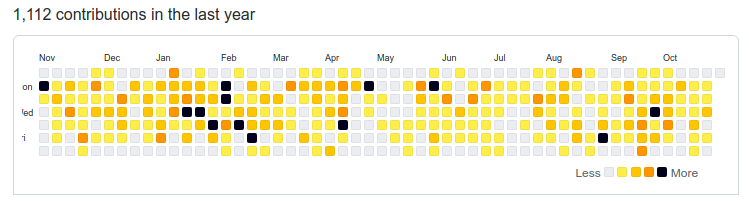
\includegraphics[width=\linewidth]{./images/github.png}

\section{Summary}
\cventry{}{With over 22 years of experience in software development, I am deeply passionate about compilers and data science. My expertise spans multiple programming languages including Python, C++, and JavaScript, applied across backend, frontend, DevOps, and packaging. I have also contributed as a Research Software Engineer (RSE) to scientific projects in transportation engineering and public health. I have contributed to renowned open-source projects such as PyTorch, ibis-framework, and the Jupyter ecosystem. I have developed and maintained diverse tools and libraries for DevOps, compilers, and automation, using advanced technologies like LLVM, PostgreSQL, Docker, OpenAI ChatGPT API, hugging face, etc. As a leader of Open Science Labs, I foster a community dedicated to open science and open source software. I have also been working as a teaching assistant in Data Science and Programming courses}{}{}{}{}{}


\section{Education}

\cventry{2015--2016}{Transportation Engineering}{Universidade Federal de Santa Catarina}{Florianópolis/Brazil}{\textit{Master's degree (interrupted)}}{}  % arguments 3 to 6 can be left empty

\cventry{2004--2005}{Information Technology}{Faculdade Eniac}{Guarulhos/Brazil}{\textit{Lato Sensu Post-Grad}}{}

\cventry{2003--2004}{Database Technology}{Faculdade Eniac}{Guarulhos/Brazil}{\textit{Associate's degree}}{}


\section{Experience (last 10 years)}

\cventry{2024--Present}{Teaching Assistant}{WorldQuant University}{Part-time}{}{Teaching Assistant in the course 'Applied Data Science Lab', Database Management, Data Cleaning and Preprocessing, Regression and Classification Modeling, Data Visualization, Ethics in Machine Learning, Business Insight and Intelligence.}

\cventry{2024--Present}{Teaching Assistant}{The GRAPH Courses}{Part-time}{}{Teaching Assistant in the course 'Python Basics and Beyond: Intro to Data Analysis with Python', focusing on topics such as Fundamentals of Python, Pandas, Plotly, Quarto Dashboards, and GitHub.}

\cventry{2015--Present}{Executive Director}{Open Science labs (OSL)}{Part-time}{}{At Open Science Labs (OSL), my role spans devops, community management, and program coordination. I established the Incubator and Open Source Internship Programs, enhancing our outreach and significantly impacting the open-source community. OSL has thrived successfully participating in the Google Summer of Code through NumFOCUS, with four students completing their projects to date. The Internship Program has also flourished, aiding seven individuals in completing their projects. I currently manage 16 projects in incubation and seven affiliated projects. My efforts include securing two grants from the Python Software Foundation, providing mentorship to recipients, and fostering various internal mentorship initiatives. Currently, I am serving as a tech leader, developer, and mentor in open-source projects such as Makim, Sugar, ArxLang, SciCookie, Envers, Anamnesis.ai, etc.}

\cventry{2023--Present}{Research Software Engineer}{The GRAPH Network/LiteRev}{Part-time}{}{In the LiteRev project, I've been acting as a Tech and Team Leader, Software Architect, and DevOps engineer. In this project, we have been using technologies such as: Python, Django, scikit-learn, pacmap, optuna, hdbscan, bokeh, celery, docker-compose, CI/CD, etc}

\cventry{2022--2023}{Research Software Engineer}{The GRAPH Network}{Part-time}{}{As a server administrator, I was responsible for ensuring the servers are operating efficiently and implementing new services for internal usage. Additionally, I provided internal training to the team on topics such as git, Python tools, and best practices. I was also responsible for defining and implementing best practices for open source projects and designing the architecture for new implementations. My expertise included working with technologies such as Python, R, CI/CD, Docker, PostgreSQL, Ansible, Nginx, Apache Superset, and packaging with conda.}

\cventry{2022--2023}{Software Developer}{Inlyse}{Part-time}{}{I acted as a project leader of a homemade platform for customers where customers can manage their license keys (for Inlyse products) and manage the payments for their license through a stripe integration.
I have worked on some tools for feeding the internal pipeline for ML training models. Some of the technologies used: Python, C++, Bash, JavaScript, Ansible, Django, Docker, CI/CD, Stripe, etc.}

\cventry{2018--2021}{Software Developer}{Quansight/OSBIG}{Part-time}{}{Contributed to Open Source projects such as PyTorch, Ibis-Framework, Jupyter ecosystem, OmniSciDB. Worked on internal and client projects with technologies such as Django, Django-Rest Framework, asyncio, Bluetooth BR/EDR communication, Docker, GraphQL, Argo Workflow, etc. As extra activities, I was a member of the DEI committee, where we've organized internal events to promote and discuss topics related to diversity, equity, and inclusion, and I have also organized and facilitated weekly meetings about compilers.}

\cventry{2017--2017}{Software Packager}{Anaconda, Inc}{Contract}{}{Acted as a software packager with conda for libraries in Python, R, and Java.}

\cventry{2016--2017}{Research Software Engineer}{Fundação para o Desenvimento Científico e Tecnológico em Saúde - Fiotec}{Contract}{}{Contributed to the development of portals for visualization of influenza and dengue incidence and estimation in Brazil. Development using technologies such as Python, Javascript, pandas, bokeh, django, flask, fiona, rasterio, PostgreSQL, MapServer, Docker, etc.}

\cventry{2016--2016}{Research Software Engineer}{Fapeu - Fundação de Amparo a Pesquisa e Extensão Universitária}{Contract}{}{Contributed to a web system for analyzing the visco-elastic characteristics of pavements in laboratory tests.}

\cventry{2013--2016}{Research Software Engineer}{Fapeu - Fundação de Amparo a Pesquisa e Extensão Universitária}{Florianópolis/Brazil}{Full-time}{Analyzed international literature to investigate methods in the transportation engineering area, such as high-speed Weigh-in-Motion (WIM) and fatigue and complex modulus tests. Developed solutions using Digital Signal Processing, Machine Learning, and High Performance Computing techniques.}

\section{Volunteer Experience}

\cventry{2020--2023}{Software Reviewer, Review Editor}{PyOpenSci}{}{}{Served as a software package reviewer, review editor, and advisor for pyOpenSci.}

\cventry{2015--2016}{Chair}{SciPy Latin America}{}{}{SciPyLA Conference 2016, held between May 16 and 20, 2016, aimed to promote: science, the adoption of information technology as a tool for scientific study and, the use of Python as the main computing tool in science (https://www.scipy.lat/conf/2016/).}

\section{Languages}
\cvitemwithcomment{}{Portuguese: Native, Spanish: Fluent, English: Advanced, Italian: Basic}{}

%\section{Computer skills}
%\cvdoubleitem{category 1}{XXX, YYY, ZZZ}{category 4}{XXX, YYY, ZZZ}
%\cvdoubleitem{category 2}{XXX, YYY, ZZZ}{category 5}{XXX, YYY, ZZZ}
%\cvdoubleitem{category 3}{XXX, YYY, ZZZ}{category 6}{XXX, YYY, ZZZ}

%\section{Interests}
%\cvitem{hobby 1}{Description}
%\cvitem{hobby 2}{Description}
%\cvitem{hobby 3}{Description}

\section{Certificados}

\cvlistitem{Compilers. edX/Stanford (2021) }
\cvlistitem{Leading With Effective Communication, Inclusive Leadership Training. edX/Catalyst (2021)}
\cvlistitem{Parallel Computing with Dask. DataCamp (2018)}
\cvlistitem{Deep Learning in Python. DataCamp (2018)}
\cvlistitem{Machine Learning with Python. DataCamp (2018)}
\cvlistitem{Machine Learning with the Experts: School Budgets. DataCamp (2018)}
\cvlistitem{Unsupervised Learning in Python. DataCamp (2018)}
\cvlistitem{Importing \& Managing Financial Data in Python. DataCamp (2018)}
\cvlistitem{Supervised Learning with scikit-learn. DataCamp (2018)}
\cvlistitem{Introduction to Applied Biostatistics: Statistics for Medical Research. Osaka University / EDX (2017)}
\cvlistitem{Intro to Hadoop and MapReduce. Udacity (2016)}
\cvlistitem{Intro to Data Science. Udacity (2014)}
\cvlistitem{Machine Learning: Supervised Learning. Udacity (2014)}
\cvlistitem{Intro to Descriptive Statistics. Udacity (2014)}
\cvlistitem{Design of Computer Programs. Udacity (2012)}

%\section{Extra 2}
%\cvlistdoubleitem{Item 1}{Item 4}
%\cvlistdoubleitem{Item 2}{Item 5\cite{book1}}
%\cvlistdoubleitem{Item 3}{Item 6. Like item 3 in the single column list before, this item is particularly long to wrap over several lines.}

%\section{References}
%\begin{cvcolumns}
%  \cvcolumn{Category 1}{\begin{itemize}\item Person 1\item Person 2\item Person 3\end{itemize}}
%  \cvcolumn{Category 2}{Amongst others:\begin{itemize}\item Person 1, and\item Person 2\end{itemize}(more upon request)}
%  \cvcolumn[0.5]{All the rest \& some more}{\textit{That} person, and \textbf{those} also (all available upon request).}
%\end{cvcolumns}

% Publications from a BibTeX file without multibib
%  for numerical labels: \renewcommand{\bibliographyitemlabel}{\@biblabel{\arabic{enumiv}}}% CONSIDER MERGING WITH PREAMBLE PART
%  to redefine the heading string ("Publications"): \renewcommand{\refname}{Articles}

%\nocite{*}
%\bibliographystyle{plain}
%\bibliography{publications}                        % 'publications' is the name of a BibTeX file

%\begin{itemize}
%\item  Poster: OpenWIM - Open Science and Weigh in Motion Research. International Conference on Weigh-In-Motion 7. DOI: 10.13140/RG.2.2.19198.48961 (\url{https://www.researchgate.net/publication/311735715_OpenWIM_-_Open_Science_and_Weigh_in_Motion_Research})
%\end{itemize}


% Publications from a BibTeX file using the multibib package
%\section{Publications}
%\nocitebook{book1,book2}
%\bibliographystylebook{plain}
%\bibliographybook{publications}                   % 'publications' is the name of a BibTeX file
%\nocitemisc{misc1,misc2,misc3}
%\bibliographystylemisc{plain}
%\bibliographymisc{publications}                   % 'publications' is the name of a BibTeX file

\end{document}


%% end of file `template.tex'.
